\documentclass[a4paper,12pt]{article}
\usepackage[utf8]{inputenc}
\usepackage{graphicx}
\usepackage{amsmath}
\usepackage{hyperref}
\usepackage[a4paper, left=2cm, right=2cm, top=2cm, bottom=2cm]{geometry}
\usepackage{float}

\begin{document}

\title{Handwritten Signature Detection and Localization in Documents}
\author{Federico Iannini, Andrea Puddu, Riccardo Pitzanti \\
\small \href{https://github.com/ricp2015/signature_localization}{https://github.com/ricp2015/signature\_localization}
\\
\small Foundations of Data Science – Sapienza University of Rome}
\date{December 2024}

\maketitle

\begin{abstract}
Localizing handwritten signatures in scanned documents is useful for automating workflows in industries such as legal, banking, and archival systems. This report explores three distinct approaches to address this task: a fixed grid-based method, a selective search-based approach leveraging image features, and a state-of-the-art Faster R-CNN model. Each method is evaluated for its ability to propose and classify regions of interest, with Faster R-CNN providing the highest accuracy via end-to-end training. The pipeline integrates preprocessing techniques, including edge detection and image filters, to enhance signature localization accuracy. Results demonstrate the trade-offs between simplicity, computational efficiency, and performance across the approaches. Future work aims to further optimize region proposal strategies, explore advanced architectures and expand towards broader use cases.
\end{abstract}

\section{Introduction}
This project focuses on automating the detection and localization of handwritten signatures in scanned documents. By identifying and bounding signatures, the pipeline reduces manual labor and improves workflow efficiency in industries like legal and banking. The approach integrates machine learning, edge detection techniques, and region-based localization to handle diverse document formats and scenarios. 

\section{Related Work}

Handwritten signature localization has garnered significant attention in the field of document analysis. Wu et al.\cite{wu2021}, Cüceloğlu and Oğul\cite{cuceloglu2018} introduced object detection models specifically tailored for handwriting localization tasks. Segmentation-based approaches like those presented by Roy et al.\cite{roy2020} leverage fully convolutional networks coupled with refinement layers to enhance the precision of offline handwritten signature localization. Alaeiyan\cite{alaeiyan2022} explored the application of deep learning architectures in signature verification systems. The use of selective search for bounding box initialization, as proposed by Uijlings et al.~\cite{victor2013}, facilitates dynamic region identification by leveraging image features.

\section{Dataset}
The dataset, SignverOD, consists of 2765 scanned document images with 7103 bounding boxes annotated across four categories: handwritten signatures, initials, redactions, and dates. For this project, the focus is solely on the "signature" category. These documents are sourced from diverse repositories, including Tobacco800, NIST.gov Special Database, a bank checks dataset, and GSA lease documents. All documents in the dataset vary in size, with bounding box annotations provided in normalized coordinates relative to document dimensions. The dataset is split into 1991 training images, 221 for validation, and 553 for testing, with 4451 bounding boxes specifically annotated as signatures. To further support the model, non-signature crops are generated by masking annotated signature regions and extracting random patches, creating a balanced dataset necessary for training a binary classifier.

\section{Pipeline Implementation}
The pipeline is designed to pre-process data, train models, and localize signatures. Basic steps include:

\subsection{Data Pre-processing}
\begin{itemize}
    \item \textbf{Dataset Download}: The dataset is sourced from Kaggle\cite{dataset} and corrected to address inconsistencies (see:~\cite{dataset_fix}). Training and testing files are merged to enable a custom data split.
    \item \textbf{Cropping Signatures}: Images are cropped to bounding boxes around their respective annotated signatures.
    \item \textbf{Resizing}: Cropped signatures are resized to a uniform dimension to standardize input for the CNN. This uniform dimension is obtained by computing the mean height and width of all the documents (734x177 pixels).
    \item \textbf{Non-Signature Generation}: Using masked images, non-signature regions are extracted, avoiding overlap with annotated signatures.
    \item \textbf{Image Pre-processing}: Edge detection techniques (Canny, Sobel, Laplacian), Gaussian filtering, binary mask thresholding, or no pre-processing can be applied as specified.
\end{itemize}

\subsection{Model Training}

The goal of the model is to classify sections of a document as either containing a handwritten signature or not. Given that the input data are images, we used a CNN structure. The architecture used in this project, shown in Figure~\ref{fig:cnn_architecture}, is a simple model consisting of convolutional, pooling, and dense layers: \begin{itemize} \item \textbf{Convolutional Layers}: Extract spatial features from the input image using filters, followed by a Leaky ReLU activation function. \item \textbf{Max-Pooling Layers}: Reduce the spatial dimensions of the feature maps while retaining the most salient information. \item \textbf{Dense Layers}: Fully connected layer maps the extracted features to a binary classification output for which the sigmoid activation function is used. \end{itemize}

Deeper architectures (e.g., additional convolutional layers and dropout) were tested, but this configuration was chosen for its balance of efficiency and performance, achieving approximately 97\% accuracy and a low binary cross-entropy loss.
\begin{figure}[H]
    \centering
    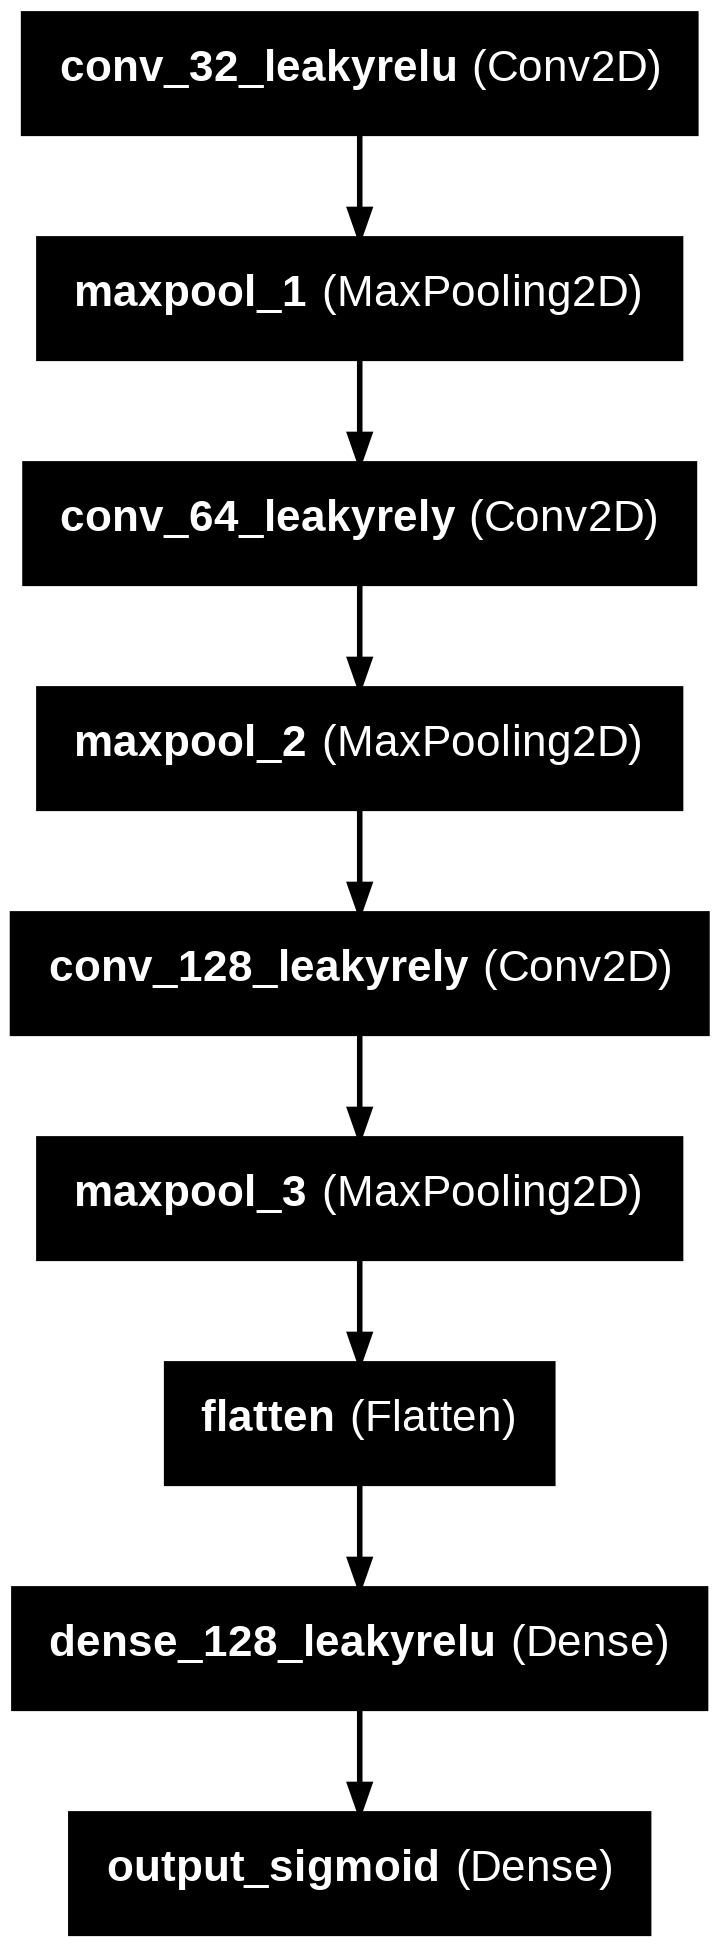
\includegraphics[scale=0.17]{net.png}
    \caption{CNN Architecture used for Signature Detection.}
    \label{fig:cnn_architecture}
\end{figure}

\subsection{Region Proposal and Classification}
Bounding box proposals during testing are generated using either a static grid-based method or a selective search-based approach. The first method divides the document into uniform grid regions and passes each region to a CNN classifier, which determines whether it contains a signature. While simple, this approach is inefficient, as it does not adapt to document features and processes many irrelevant regions, leading to higher computational costs.

The selective search-based method improves upon this by introducing a dynamic region proposal mechanism. Instead of dividing the document into a fixed grid, selective search identifies potential regions of interest dynamically. A set of bounding boxes is initialized at random coordinates within ink-detected parts of the document. The size and aspect ratio of these bounding boxes are scaled relative to a precomputed "base dimension", derived from the average dimensions of annotated bounding boxes in the training dataset (see Resizing, in 4.1). To introduce variability, oscillating factors are applied to the width and height of the base dimension, resulting in varied bounding boxes. 

Each bounding box is classified by the CNN, which determines whether it contains a signature. Only bounding boxes with classification confidence scores exceeding a specified threshold ($\ge$ 90\%) are retained.


\section{Faster R-CNN}
A Faster R-CNN model, a state-of-the-art object detection framework, was implemented to assess its suitability for the task of handwritten signature localization. The model combines region proposal and classification into an end-to-end trainable system and was fine-tuned on the SignverOD dataset.

\section{Performance Evaluation}
Performance is evaluated for each method using precision, recall, F1 score, and Intersection over Union (IoU) metrics. A bounding box is classified as a true positive if its IoU with the ground truth exceeds 0.4. The iterative localization process ranks regions based on confidence scores, removing overlapping predictions through non-maximum suppression.

\section{Results}


\begin{table}[ht]
\centering
\begin{tabular}{|l|c|c|c|c|}
\hline
\multicolumn{5}{|c|}{\textbf{Method 1: Fixed Grid-Based Approach}} \\ \hline
\textbf{Preprocessing Technique} & \textbf{Precision} & \textbf{Recall} & \textbf{F1-Score} & \textbf{Mean IoU} \\ \hline
no preprocessing              & 0.1654             & 0.3158          & 0.2171            & 0.4168            \\ \hline
binary mask thresholding            & 0.2879             & 0.3707          & 0.3241            & 0.3845            \\ \hline
canny                 & 0.2964             & 0.4029          & 0.3416            & 0.3878            \\ \hline
sobel                 & 0.6818             & 0.1531          & 0.2500            & 0.4060            \\ \hline
gaussian              & 0.1916             & 0.3380          & 0.2446            & 0.3631            \\ \hline
laplacian             & 0.4368             & 0.3290          & 0.3753            & 0.3887            \\ \hline
\end{tabular}

\vspace{0.5cm}

\begin{tabular}{|l|c|c|c|c|}
\hline
\multicolumn{5}{|c|}{\textbf{Method 2: Selective Search-Based Approach}} \\ \hline
\textbf{Preprocessing Technique} & \textbf{Precision} & \textbf{Recall} & \textbf{F1-Score} & \textbf{Mean IoU} \\ \hline
no preprocessing          & 0.1109             & 0.4785          & 0.1800            & 0.4427            \\ \hline
binary mask thresholding       & 0.3770             & 0.3366          & 0.3557            & 0.4044            \\ \hline
canny             & 0.1956             & 0.3757          & 0.2572            & 0.3951            \\ \hline
sobel             & 0.4118             & 0.1429          & 0.2121            & 0.4094            \\ \hline
gaussian          & 0.1297             & 0.5286          & 0.2083            & 0.4075            \\ \hline
laplacian         & 0.2177             & 0.3939          & 0.2804            & 0.4113            \\ \hline
\end{tabular}
\vspace{0.5cm}

\begin{tabular}{|l|c|c|c|c|}
    \hline
    \multicolumn{5}{|c|}{\textbf{Method 3: Faster R-CNN}} \\ \hline
    \textbf{Preprocessing Technique} & \textbf{Precision} & \textbf{Recall} & \textbf{F1-Score} & \textbf{Mean IoU} \\ \hline
    canny             & 0.8991             & 0.5542          & 0.5218            & 0.6319            \\ \hline
    \end{tabular}
\caption{\centering Evaluation Metrics and Mean IoU for Methods 1 (Fixed Grid-Based Approach) and 2 (Selective Search Approach) under Different Preprocessing Techniques. Method 3 (Faster R-CNN) is evaluated using only Canny preprocessing.}
\end{table}

Table 1 summarizes the performance of the two proposed methods under various preprocessing techniques. The results indicate that preprocessing, whether by applying no modifications, edge detection, or binary mask thresholding, has a significant impact on performance metrics. For Method 1, Laplacian filtering achieves the best F1-score (0.3753), while for Method 2, binary mask thresholding provides the highest F1-score (0.3557). Overall, the mean IoU values remain in a moderate range (approximately 0.36–0.44). Notably, Method 2 achieves the highest mean IoU (0.4427) without preprocessing, but its corresponding F1-score is considerably lower (0.1800).  The two methods show comparable performance in terms of precision and recall, but Method 2 significantly reduces execution time. So, despite the slight decrease in F1-score, the improved mean IoU and faster runtime make Method 2 preferable in many applications. However, as highlighted earlier, a more advanced detector such as Faster R-CNN surpasses these two-step pipelines in both accuracy and adaptability.

\section{Future Work}
A core area for improvement is the refinement of region proposal methods, which could involve leveraging existing algorithms or developing new, more effective ones. Dynamic approaches, such as adaptive bounding box generation, offer significant potential for improving Intersection over Union (IoU) metrics, as static bounding box sizes often fail to accommodate varying signature dimensions. Another promising direction is the adoption of advanced deep learning models like YOLO and Transformer-based architectures. Additionally, the system's functionality could be expanded to include broader use cases, such as forgery detection.

\section{Roles}
\begin{itemize}
    \item \textbf{Data pre-processing, fixed grid-based algorithm implementation}: Federico, Riccardo
    \item \textbf{Selective search-based algorithm and CNN model}: Federico
    \item \textbf{Performance evaluation and report writing}: Riccardo
    \item \textbf{Faster R-CNN}: Andrea
\end{itemize}

\begin{thebibliography}{9}
\bibitem{wu2021} Wu, Yuli, Yucheng Hu, and Suting Miao. "Object Detection Based Handwriting Localization." \textit{arXiv preprint} (2021). \url{https://arxiv.org/pdf/2106.14989}.
\bibitem{cuceloglu2018} Cüceloğlu, İlkhan, and Hasan Oğul. "Detecting handwritten signatures in scanned documents." \textit{ResearchGate} (2018). \url{https://www.researchgate.net/publication/326271482}.
\bibitem{alaeiyan2022} Alaeiyan, Mehdi. "Handwritten Signature Verification System Using Deep Learning." \textit{PhilArchive preprint} (2022). \url{https://philarchive.org/archive/ALAHSV}.
\bibitem{roy2020} Roy, Ankita, et al. "FCN+RL: A Fully Convolutional Network followed by Refinement Layers to Offline Handwritten Signature Segmentation." \textit{arXiv preprint} (2020). \url{https://arxiv.org/pdf/2005.14229}.
\bibitem{victor2013} Uijlings, J.R.R., et al. "Selective Search for Object Recognition." \textit{International Journal of Computer Vision} (2013). \url{https://ivi.fnwi.uva.nl/isis/publications/2013/UijlingsIJCV2013/UijlingsIJCV2013.pdf}.
\bibitem{dataset} "SignverOD Dataset." Kaggle. \url{https://www.kaggle.com/datasets/victordibia/signverod}.
\bibitem{dataset_fix} "Fixing the SignverOD Dataset." Kaggle. \url{https://www.kaggle.com/code/alexhorduz/fixing-signverod-dataset}.
\end{thebibliography}



\end{document}
